% !TeX root = ../thesis.tex

\chapter{\acf{TPM}}
\label{sec:tpm}

With the \ac{TPM} the \ac{TCG} specifies a system component designated for security\-/related functions, providing the ability to establish trust in a system \cite{microsoft-windows-trusted-platform-module-overview}.
Its implementation can be accomplished through dedicated hardware or by using the \ac{CPU}'s isolated \ac{SMM} \cite[Section 9.3]{tcg-tpm-library-part1-architecture}.
Asides from generating and securely storing cryptographic keys, the \ac{TPM} can be used for system integrity measurements.
Boot code is measured into the \ac{TPM} by the \ac{PF}, providing evidence over the initialization process and making it possible to detect deviations \cite{microsoft-windows-trusted-platform-module-overview}.

\section{\acfp{PCR}}
\label{sec:tpm:pcr}

\cite{tcg-tpm-library-part1-architecture} defines \acp{PCR} to store the system integrity measurements.
The registers can only be modified in two ways: either through a complete \ac{TPM} reset or by extending their values.
Extending a \ac{PCR} is done by concatenating the hashed measurements together with the current \ac{PCR} values to form the new contents, as depicted in \autoref{eqn:pcr-extend}.
This creates a chain of measurements where from one diverging measurement on, all subsequent \ac{PCR} extensions result in entirely different values.

\begin{equation}
    PCR[i]_{(new)}\:=\:Hash(PCR[i]_{(old)}\:||\:Hash(Measurement))
    \label{eqn:pcr-extend}
\end{equation}

The \ac{TPM} is a passive system component, relying on the host processor to perform measurements and extend the \acp{PCR}.
The measurement chain starts with a point called the \ac{CRTM}, consisting of the first instructions executed to establish a chain of trust.
A root of trust in a system is an element that must be trusted as its behavior is non\-/verifiable \cite{tcg-tpm-library-part1-architecture}.
\cite[3.2.2]{tcg-pc-client-platform-firmware-profile-spec} requires this chain to start in an immutable portion of the \ac{PI} process, the \ac{SRTM}.
\cite[3.2.3.1]{tcg-pc-client-platform-firmware-profile-spec} defines the \ac{PF} to be composed of a Boot Block and the \ac{UEFI} firmware, the Boot Block consists of the \ac{SEC} and \ac{PEI} phase as well as the \ac{IBB}.
The \ac{IBB} forms the \ac{SRTM}, while the rest of the \ac{UEFI} firmware is only part of the chain of trust by being measured from the \ac{SRTM}.
The \ac{RTM} can either start with the \ac{SRTM} measuring itself or a \ac{H-CRTM} measuring the \ac{SRTM}.
It falls under the responsibility of the \ac{PF} to perform the integrity measurements \cite{tcg-pc-client-platform-firmware-profile-spec}.
Different parts of the boot process are measured into separate \acp{PCR}.
\autoref{fig:pf-measurement-flow} shows a high\-/level measurement flow.
\autoref{tab:pcr-usage} on \pageref{tab:pcr-usage} shows \ac{PCR} indexes relevant to this thesis and the type of measurements performed to extend them.

Interaction with the \ac{TPM} is done via a well\-/defined interface.
For external chips, this is done over hardware buses such as \ac{LPC} or \ac{SPI}.
\ac{TCG} specifies the \nameref{lst:tcg2-protocol} for the \ac{UEFI} environment, providing an abstracted communication interface independent of the underlying implementation.

\begin{figure}[htb]
    \centering
    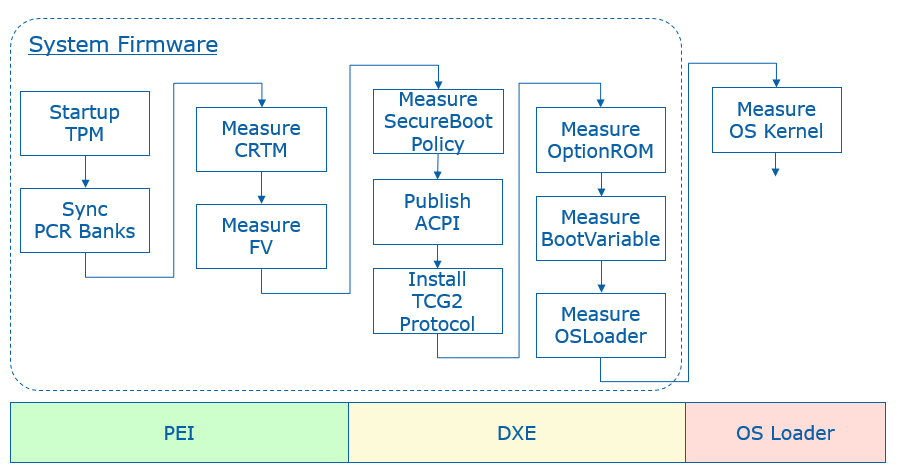
\includegraphics[width=1.0\textwidth]{tpm/tpm_measurements}
    \caption[\acs{PF} Measurement Flow]{\acs{PF} Measurement Flow (taken from \cite[Figure 3]{tianocore-trusted-boot-chain})}
    \label{fig:pf-measurement-flow}
\end{figure}

\begin{table}[htb]
    \centering
    \begin{tabularx}{1.0\textwidth}{cX}
        \toprule
        \textbf{\acs{PCR} Index}    & \textbf{Measurements}                                                                                    \\
        \midrule
        \textbf{0}                  & \acs{SRTM}, \acs{BIOS}, Host Platform Extensions, Embedded Option\-/\acsp{ROM}, and \acs{PI} Drivers     \\[\defaultaddspace]
        \arrayrulecolor{gray}
        \midrule
        \textbf{1}                  & Host Platform Configuration                                                                              \\[\defaultaddspace]
        \midrule
        \textbf{2}                  & \acs{UEFI} driver and application Code                                                                   \\[\defaultaddspace]
        \midrule
        \textbf{3}                  & \acs{UEFI} driver and application Configuration and Data                                                 \\[\defaultaddspace]
        \midrule
        \textbf{4}                  & \acs{UEFI} Boot Manager Code (usually the \acs{MBR}) and Boot Attempts                                   \\[\defaultaddspace]
        \midrule
        \multirow{2}{*}{\textbf{5}} & Boot Manager Code Configuration and Data (for use by the Boot Manager Code) and \ac{GPT}/Partition Table \\ \addlinespace[1.0\defaultaddspace]
        \midrule
        \textbf{6}                  & Host Platform Manufacturer Specific                                                                      \\[\defaultaddspace]
        \midrule
        \textbf{7}                  & Secure Boot Policy                                                                                       \\[\defaultaddspace]
        \midrule
        \textbf{8}                  & First \acsu{NTFS} boot sector (volume boot record)                                                       \\[\defaultaddspace]
        \midrule
        \textbf{9}                  & Remaining \acsu{NTFS} boot sectors (volume boot record)                                                  \\[\defaultaddspace]
        \midrule
        \textbf{10}                 & Boot Manager                                                                                             \\[\defaultaddspace]
        \midrule
        \textbf{11}                 & BitLocker Access Control                                                                                 \\
        \arrayrulecolor{black}
        \bottomrule
    \end{tabularx}%
    \caption[\acs{PCR} Usage]{\ac{PCR} Usage (taken from \cite[Table 1]{tcg-pc-client-platform-firmware-profile-spec} and \cite[Table 9-2]{windows-internals-6-part2})}%
    \label{tab:pcr-usage}%
\end{table}


\section{Sealing/Unsealing}

The chain of measurements can be used to attest that the system is in a trusted state.
The \ac{TPM} can be given data, for example, a cryptographic key, in a state that is assumed to be trusted.
This state is reflected by the current \acp{PCR}, consisting of the collection of lead\-/up measurements.
The \ac{TPM} then seals the data with a policy that describes which \ac{PCR} indexes to use and/or proof of authentication through a \ac{PIN} or passphrase.
The data can then only be unsealed on subsequent boots when the system is in the same trusted state that it was in when the data was sealed.
Any modification of the boot code will be reflected in a deviation of \ac{PCR} values leaving the \ac{TPM} unable to unseal the data \cite[Section 3.3.6]{trusted-computing-platforms}.